\documentclass[11pt]{article}
\usepackage[margin=1in]{geometry}
\usepackage{booktabs}
\usepackage{amsmath}
\usepackage{amssymb}
\usepackage{enumitem}
\usepackage{float}
\usepackage{graphicx}
\usepackage{tabularx}
\usepackage{tikz}
\usepackage[hidelinks]{hyperref}
\usetikzlibrary{arrows.meta,fit,positioning,shapes.geometric}
\newcommand{\pra}{\mathrm{PRA}}
\newcommand{\refhandle}{\mathrm{REF}}
\newcommand{\kv}{\mathrm{KV}}
\newcommand{\q}{\mathbf{Q}}
\newcommand{\kmat}{\mathbf{K}}
\newcommand{\vmat}{\mathbf{V}}

\newcolumntype{P}[1]{>{\raggedright\arraybackslash}p{#1}}
\newcolumntype{Y}{>{\raggedright\arraybackslash}X}
\setlength{\emergencystretch}{3em}
\definecolor{prablue}{HTML}{245A8D}
\definecolor{pragreen}{HTML}{2D7A68}
\definecolor{pragold}{HTML}{A66A18}
\definecolor{pragray}{HTML}{5F6B76}
\definecolor{pralight}{HTML}{EEF3F7}
\tikzset{
  sysnode/.style={draw=prablue, fill=pralight, rounded corners=2pt, align=center,
  minimum height=8mm, inner sep=4pt, font=\small}, cachenode/.style={draw=pragreen,
  fill=green!6, rounded corners=2pt, align=center, minimum height=8mm, inner sep=4pt,
  font=\small}, datanode/.style={draw=pragold, fill=orange!7, rounded corners=2pt,
  align=center, minimum height=8mm, inner sep=4pt, font=\small},
  sysflow/.style={-{Stealth[length=2mm]}, thick, draw=pragray}
}

\title{Progressive Retrieval Attention: Bounded Sparse Native-KV for Addressable Logical
Memory}
\author{Jorge Sim\~ao\\EInnovator R\&D, Portugal}
\date{\today}
\hypersetup{
  pdftitle={Progressive Retrieval Attention: Bounded Sparse Native-KV for Addressable
  Logical Memory}, pdfauthor={Jorge Simao}
}

\begin{document}
\maketitle

\begin{abstract}
Transformer context windows typically force logical memory and active attention to grow
together. Progressive Retrieval Attention (PRA) separates them.
A large logical memory is encoded once as layer-native key/value (K/V) state;
compact gists route each query to a bounded subset; and only the selected,
full-detail K/V participates in the model's ordinary attention operation.
The gist therefore serves as metadata for selection,
not as a compressed surrogate for the token state that attention ultimately reads.

We evaluate this mechanism in controlled standalone transformers.
The central repair is to encode contiguous context before slicing smaller routing units;
independently encoded microchunks discard the historical context required for faithful
K/V. After this repair, fixed selection breadth over split labels 64--256 (63--255
addressable source units) reduces the active fraction from 17.9--18.7\% to 4.4--4.9\%
while retaining essentially all measured dense-context benefit in the small model.
A fixed-fraction reanalysis isolates router quality from increasing sparsity:
selecting approximately 12.5\% of references yields annotated target coverage of
0.756/0.772/0.762 on HotpotQA-derived examples and 0.794/0.803/0.800 on QASPER-derived
examples at split labels 64/128/256. Under a hard 32-token attention-axis limit,
PRA addresses a 184-token displaced prompt head inside 192 logical tokens,
achieving loss 1.0567 versus 1.2287 for truncation, with no operation-limit violations.
Exact Split-256 routing over 255 candidates requires 5.5--11.6\,ms after index
construction in this prototype.

In a separate pretrained Qwen3 8B--32B MLX calibration,
selected native K/V matches all selected-text sequences at 8B/14B and 13/15 at 32B while
the full-versus-selected answer-quality sign changes across model size. At 8B,
selected detail remains approximately 39.6\,MiB as full native K/V grows from
1{,}152\,MiB at 8K to 4{,}608\,MiB at 32K. These results establish sparse transport of
selected native K/V and bounded execution over larger logical memory.
They do not establish unrestricted question answering,
arbitrary positional extrapolation, or produ 
ction serving efficiency.
\end{abstract}

\section{Introduction}

Self-attention layers in transformer architectures face a well-known tension:
the quadratic cost of attention forces a trade-off between the size of the logical
context that can be addressed and the number of key/value (K/V) tokens that must be
processed in any single operation. Vanilla dense self-attention implementations
treat these two sets as identical: all previous K/V tokens, from the beginning of the
sequence up to the maximum context length, are both addressable and active.
This design is simple, but it makes active computation, device-resident state, and
memory use grow with the entire context, even when the next-token prediction depends
on only a few earlier regions.

In this paper, we introduce \textbf{Progressive Retrieval Attention} (PRA), a variant
of self-attention (SA) that separates these two quantities: which K/V tokens can
potentially be addressed and which are actually selected for each next-token inference
step. The motivation is that a context may contain many more tokens than are needed for
a given prediction, and the relevant subset of K/V vectors may change from one token to
the next. PRA stores historical model state outside the current token stream, organizes
that state into logical chunks, regions, or records, and applies a selection criterion
to identify the relevant chunks. The criterion first explored and reported in this paper
uses compact routing gists derived from the token keys (K) of candidate regions.

Selected regions are materialized in full: if a region is selected, all token K/V pairs
in that region are selected. This property is important because self-attention weights
tend to be highly localized, with occasional long-distance dependencies. When chunking
creates overlapping regions, duplicate token K/V pairs are removed.

PRA combines the selected memory K/V with the direct-context K/V in the same attention
\textsf{softmax} operation at each layer. PRA layers can be used when designing new
transformer models or can selectively replace dense SA layers in pretrained models.
In PRA, context tokens can come from three sources: prompt-prefill or previously generated
tokens; pre-encoded documents referenced in the prompt through markers
(\texttt{\_\_ref}); and a generation-rollover pseudo-document (\texttt{\_\_head})
created automatically when the context exceeds the configured limit. The maximum number
of selected K/V tokens from each source can be configured so that their total does not
exceed the model's supported limit.

In short, the workflow of a PRA-enabled model is as follows:

\begin{center}
\fbox{large logical memory}
$\rightarrow$ \fbox{contextual encoding} $\rightarrow$ \fbox{compact routing gists}
$\rightarrow$ \fbox{selected regions} $\rightarrow$ \fbox{full-detail native K/V}
$\rightarrow$ \fbox{bounded attention}.
\end{center}


PRA differs from traditional \emph{Retrieval-Augmented Generation} (RAG)
\cite{gao2023ragsurvey}, and from the more recent proposal
\emph{Cache-Augmented Generation} (CAG) \cite{chan2024cag}.
RAG retrieves text chunks and inserts them into a prompt as additional context.
Documents must be preprocessed and ingested, typically by chunking and encoding them with
an external embedding model and then storing their embeddings in a vector database.
Searching for relevant chunks requires encoding the query with the same embedding model
\cite{lewis2020rag,guu2020realm,borgeaud2022retro}. PRA instead determines how
already-encoded model state enters attention by using the transformer's native,
layer-specific Q/K/V representations.

CAG similarly proposes using a precomputed model-native K/V cache for documents. However,
CAG admits complete document caches into attention and, unlike RAG, provides no retrieval
mechanism for choosing which documents to use for each prompt. PRA selects cached K/V at
the granularity of logical chunks, thereby combining properties of RAG and CAG. RAG can
also be composed with PRA: a retriever may choose documents or document parts, while PRA
controls sparse access within their cached state.

PRA is also distinct from sparse self-attention over a single admitted sequence and from
methods that permanently discard or merge token K/V. In PRA, cached K/V remains
addressable and is used unmodified when selected. The routing representation---the chunk
gists---is compressed, but the selected K/V payload is not. Thus, provided that chunk
retrieval is accurate and sufficient, PRA is lossless with respect to the materialized
K/V payload. Existing sparse SA layers address only the current admitted sequence,
whereas PRA integrates K/V from externally referenced documents into the same attention
system.

The central claim of this paper is:

\begin{quote}
PRA can make a memory that is substantially larger than the K/V set active in any one
model operation logically visible to a decoder, while preserving the full-detail native
K/V of the selected regions. With sufficiently accurate selection, models can reference very
long contexts and external documents through an integrated interface while operating on
much smaller active contexts and retaining comparable performance.
\end{quote}


Several component mechanisms used in PRA have been explored in other proposals. Content
routing, external memory, native-K/V caching, and bounded attention all have substantial
prior art. PRA's contribution is their particular contract: addressable logical memory;
support for external references and completion in an integrated framework; compact
routing metadata; selected full-detail, layer-native K/V; a configurable hard bound on
context size; and encoding granularity separated from routing granularity. This
combination lets the logically available context grow without requiring every available
token, or a compressed surrogate of every token, to enter a single attention operation.

PRA's main motivations and contributions can be summarized as follows:

\begin{itemize}
  \item Support for logical contexts larger than the underlying model's native context window.
  \item Economical use of compute and memory by limiting the active context to what is
  needed for each prediction.
  \item Reuse of stored document encodings across prompts and sessions.
  \item The global reach of self-attention combined with the subquadratic active-context
  scaling associated with local attention.
  \item Better use of the memory--storage--compute hierarchy by offloading temporarily
  inactive K/V state to lower tiers.
\end{itemize}


The primary causal tests use small, controlled PyTorch models rather than a production
serving stack; a separate pretrained MLX calibration tests only transport compatibility
and payload accounting. The experiments separate four issues that would otherwise be
easy to confuse: whether cached native K/V carries useful detail,
whether the router finds the annotated source, how quality changes as selection becomes
sparse, and whether every underlying model call remains within a declared length bound.

\begin{table}[H]
\centering
\footnotesize
\caption{Headline results. The rows separately address representation fidelity,
sparse systems scaling, routing quality, bounded execution, and device residency.}
\label{tab:headline}
\begin{tabularx}{\textwidth}{P{0.22\textwidth}P{0.31\textwidth}Y}
\toprule
Finding & Measurement & Meaning \\
\midrule
Fragmentation repair & Split-64 oracle RCB: .546$\rightarrow$.996
(HotpotQA-derived), .748$\rightarrow$.999 (QASPER-derived) & Encode contiguous context
before exposing smaller routing views \\
Fixed-$k$ sparse scaling &
  $k=8$ keeps 11--13 physical K/V tokens active; active fraction
falls .179$\rightarrow$.044 and .187$\rightarrow$.049 from split 64 to split 256 &
  Accessible
memory grows while the selected payload remains approximately flat \\
Fixed-fraction quality scaling & Coverage at about 12.5\% selection is
.756/.772/.762 and .794/.803/.800 at split labels 64/128/256 &
  Fixed-$k$ decline partly reflects
increasing sparsity rather than routing collapse \\
Bounded logical context &
  192 logical tokens, 184-token \texttt{\#\_\_head}; maximum source
input 20 and maximum combined attention K/V 28 under a limit of 32 &
  Logical memory can exceed one native
operation without violating the configured bound \\
CPU-resident detail K/V &
  At split 256 (255 source units), .734--3.420 MiB leaves GPU; loss and selection are
unchanged; warm overhead is 4.0--13.5 ms &
  Sparse selection becomes a measured device-capacity
tradeoff when inactive detail is offloaded \\
Measured capacity effect &
  QASPER-derived routed RCB at split 256 (255 source units): .908 tiny versus 1.000
small &
  Some degradation at large split labels reflects tested model/router capacity rather
  than transport \\
\bottomrule
\end{tabularx}
\end{table}

The headline is not that one operating point solves the long-context problem.
It is that logical memory, routing resolution, active native K/V,
and device residency are separately controllable and separately measurable.

The remainder of the paper first explains the mechanism and then evaluates controlled
transport, routing, scaling, and bounded execution before presenting the pretrained
calibration and systems costs separately.
Positional extrapolation is treated only as a boundary here;
RoPE-specific semantics belong to the companion position paper.
Pretrained architecture retrofit, iterative multi-hop retrieval, multi-gist routing,
and production serving are separate extensions.


\section{PRA Mechanism}
\label{sec:mechanism}

\subsection{PRA Overview}
\label{sec:overview}

PRA assumes that an application or user may need a potentially long context, such as one
or more documents or a long conversation, while the main prompt---for example, a question
or task description---and the newly generated tokens at each turn form a relatively short
tail. PRA processes this tail with conventional dense self-attention: all cached K/V tokens
in the tail are selected at each PRA layer. For earlier context, additional routing
mechanisms choose which cached K/V entries participate in attention.

\begin{figure}[H]
\centering
\input{figures/context_selection.tikz.tex}
\caption{Overlapping chunks and one per-token PRA selection. Each document and the
rollover \texttt{\#\_\_head} is chunked in its own local coordinate space. Chunk spans share
one row and adjacent chunks overlap by approximately 30\%; dashed vertical pairs delimit
the middle chunks $A_2$, $B_2$, and $H_2$. Every token in a selected chunk is retained.
Selected spans are merged into the solid-green union below, so overlapping tokens appear
exactly once. The blue direct tail is selected in full, while gray token spans remain
addressable but inactive in this attention operation.}
\label{fig:context-selection-line}
\end{figure}

PRA treats the context as a contiguous stream but partitions it into regions or blocks and
selects which regions enter attention for each generated token. Specifically, the
experiments reported in this paper use overlapping, fixed-size logical chunks, somewhat
resembling the chunking used during RAG ingestion. For every chunk at each PRA model layer,
metadata records the chunk's location and span, its routing information, and links to the
corresponding cached K/V entries. The routing information consists of one or more semantic
gists derived from those entries.
Figure~\ref{fig:architecture-pipeline} illustrates how overlapping chunks
are selected to produced deduplicated non overlapping span. 

We evaluate several ways to compute gists, including the K vector of the chunk's final
token, the mean K vector across all entries in the chunk, and other constructions. 
The gists of documents are computed once at ingestion time and cached for reused as index.
At decoding time, the current query vector (Q) is scored with gist matches, and a budget-aware
ranker selects a subset of chunks and their corresponding K/V spans. A metadata-only chunk
merger removes duplicate entries created by consecutive overlapping chunks and produces a
unique set of nonoverlapping spans, each defined by a starting offset and length. The
original K/V slices for these spans are concatenated and combined with the direct K/V
entries from the context tail in a single attention operation. 

When multiple gists per chunk are used, different multiple policies can be used to computed 
spans inside the chunks. The simplest approach is to create sub-chunks and compute the gists
for each subchunks. When a subchunk is matched the full parent chunk is selected and given to
and considered for materialization.

Formally, we can write the context of a completion as: $\{ D_i\}$ --- a set of documents, $\_\_head$,
and the direct or tail context $C$. Each $D_i$ is split in chunks of fixed size $\{ d_i^j \}$, 
which corresponding to a span with start and end offset inside the document as: $(d_i^j[0], d_i^j[l_i])$.


Diagram in figure~\ref{fig:architecture-pipeline}, show the complete workflow of a PRA enabled model.

\begin{figure}[H]
\centering
\resizebox{\textwidth}{!}{%
\input{figures/architecture_pipeline.tikz.tex}%
}
\caption{\textbf{PRA compresses the search representation,
not the selected memory payload.}
Contextual encoding produces native state, compact gists select addresses,
and full-detail
token K/V enters bounded attention.}
\label{fig:architecture-pipeline}
\end{figure}

PRA separates different lengths which traditionally are capture as single length:

\begin{description}[leftmargin=3.2cm,style=nextline]
\item[$L_{\mathrm{logical}}$] The amount of memory the request may logically address: direct
history plus registered external or displaced source state.
This can in principle, include an arbitrary number of documents or arbitrary length,
and a arbitraly long rollover  \texttt{\#\_\_head}.
\item[$L_{\mathrm{model\mbox{-}op}}$] The number of K/V tokens participating in one native
transformer operation. PRA has parameter to
select this quantity independently of
$L_{\mathrm{logical}}$.
\item[$L_{\mathrm{max{-}head}}$] The maximum number of K/V tokens from the rollover \texttt{\#\_\_head}.
\item[$L_{\mathrm{max{-}context}}$] The actual maximum context size supported
by the underlying model or selected by the app/user invoking the completion.
\end{description}


PRA separates three levels of granularity and corresponding policies:

\begin{itemize}
  \item encoding -- full documents are encoded up to max context size of model
  \item selection -- chunks in documents and context head are partially selected and considered
  \item routing -- one or more gists of chunks are used to select parent chunks. Ranking is used to selecte top k matches. 
  \item materialization -- subset of selected K/V entries of each select chunk.
\end{itemize}

PRA also separate the logical position of a token from the position that is
used in token embedding. Because, position is used by model when encoding
tokens K/V, caching is accounts for the fact that the position of a token
in a document needs to be shifted when reused in a prompt.


Overall, given a set of cached memory retrieved K/V $(K_M,V_M)$ and 
direct entries K/V $(K_D,V_D)$, the final operation attention operation
is defined as a modification to standard SA:

\begin{equation}
  \operatorname{PRA}(Q)=
  \operatorname{softmax}\!\left(
  \frac{Q[K_M;K_D]^\top}{\sqrt{d_h}} + M
  \right)[V_M;V_D],
  \label{eq:pra-attention}
\end{equation}

\noindent, where $M$ preserves causal and padding constraints.
The same attention scores and output projection are used for memory and direct state.
We have also experimented with cross-attention approach,
we output from direct K/V is summed with memory K/V (see appendix~\ref{app:adaptation}).
However, experimental results showed that appending rather 
than weighted sum of memory and direct values to give better results.


\subsection{Exact Routing and Whole-Chunk Budgeting}

For query vector $q$ and gist vector $g_i$, a router is used to compute a matching score.
The simplest router uses  cosine-like similarity:
\begin{equation}
  s_i = \frac{q^\top g_i}{\max(\lVert q\rVert_2\lVert g_i\rVert_2,\epsilon)},
\end{equation}

Given a set of scores, selects top-ranked chunks owners of the gist using a tensorized \texttt{topk} operation.


The set of selected chunks alone does not determine active K/V directly,
because chunks may differ in size or overlap. 
Additionally, the materialization policy decides which K/V today
include from the selected chunks considering the token budget.
Specifically, given a model or user defined token limit $L_{\max}$,
PRA setting maintain the following invariant:
\begin{equation}
  L_D + L_M + L_R \leq L_{\max},
  \label{eq:budget}
\end{equation}

\noindent, where $L_D$ is direct context, $L_M$ materialized memory, and $L_R$ a safety reserve.

\subsection{What PRA Changes, and What It Does Not}

PRA changes the set of historical K/V vector active for a query. 
It includes not only the tail of the context, but also external documents and the head
of the context. This allow token decoding to operate on a virtual K/V space.
This does imply that external storage is free, does guarantees that the router selects causal
evidence for the completion, or that it enlarges the physical positional range a pretrained model has learned.
It can reduce active attention and GPU residency while retaining a larger logical cache
elsewhere. 

Sparse-attention methods such as Longformer, BigBird, Reformer,
and Routing Transformer changes the set of K/V vector that are reachable.
\cite{beltagy2020longformer,zaheer2020bigbird,kitaev2020reformer,roy2021routing}.
KV-cache methods such as H$_2$O, SnapKV, and ClusterKV reduce retained decode state
\cite{zhang2023h2o,li2024snapkv,liu2024clusterkv}. PRA instead retains the source K/V detail outside
the active completion and uses a compact routing index to decide which full token K/V to expose.

\section{Evaluation Design}
\label{sec:evaluation}

The standalone experiments use decoder-only transformers in two controlled capacity
tiers: a tiny tier with 2.2--2.4M parameters and a small tier with 6.6--6.9M parameters.
Unless otherwise stated, comparisons use five paired seeds and 32 held-out examples per
seed. The goal is mechanism isolation, not benchmark leadership.

The datasets have different jobs:
\begin{itemize}[leftmargin=*]
\item \textbf{Synthetic reference data} creates direct, known dependence on an earlier
source span and exposes failures that natural language may hide.
\item
  \textbf{WikiText-2} checks ordinary language-model behavior and contextual integrity.
It is not used as evidence that a free-running model performs long-document QA.
\item
  \textbf{HotpotQA-derived and QASPER-derived probes} provide natural text, distractors,
and annotated source identity. Targets are controlled answer codes,
so these experiments measure evidence transport and routing coverage rather than
unrestricted QA.
\end{itemize}

Table~\ref{tab:main-config} records the configuration behind the principal split-64--256
scaling result. The scale manipulation does not add 256 independent documents:
it constructs one 255-unit source for each question and evaluates nested prefixes
repartitioned into 63, 127, or 255 addressable units.
Candidate count is therefore a routing-granularity variable,
while accessible token count is reported separately.

\begin{table}[H]
\centering
\scriptsize
\caption{Reproduction contract for the principal controlled scaling experiment.
``Final''
means the fixed terminal training step; no validation-best checkpoint selection is
used.}
\label{tab:main-config}
\begin{tabularx}{\textwidth}{P{0.19\textwidth}Y}
\toprule
Field & Frozen setting \\
\midrule
Data construction &
  HotpotQA train (4,000 constructed examples) or QASPER train (200), with a
deterministic 80/10/10 internal split and 3,200/160 optimization examples;
separate frozen
64-question evaluation source, first 32 questions evaluated per seed;
nested 63/127/255-source-unit
versions preserve question IDs and answers. Construction/evaluation seeds are
31,337/72,991
(HotpotQA) and 44,321/82,811 (QASPER) \\
Tokenizer and target &
  Dataset-specific BPE, target vocabulary cap 8,000, minimum frequency 2
(realized vocabulary: HotpotQA 8,000; QASPER 7,339);
cross-entropy supervises only the first
answer token at the final prompt position, with all other labels masked \\
Tiny tier &
  width 128, 4 heads, 2 layers, feed-forward width 256, batch 8, 200 AdamW steps \\
Small tier &
  width 256, 4 heads, 4 layers, feed-forward width 768, batch 4, 300 AdamW steps \\
Shared optimization & learning rate $7\!\times\!10^{-4}$, weight decay 0, dropout 0,
gradient-norm clip 1.0, maximum sequence length 768; final-step checkpoint \\
Pairing &
  seeds 1, 7, 21, 42, 87; identical question order and answer labels across scale
  variants \\
PRA conversion &
  inference-only, weight-preserving conversion from the trained self-attention
model; contextual \texttt{native\_slice}; global source positions and historical
direct-tail positions \\
Routing &
  one mean-pooled key gist per unit; query is the newest direct token's projected query;
cosine-like exhaustive ranking; whole-unit admission;
$k=8$ is materially evaluated in the small
tier, while full-ranking cutoffs $k=8,16,32$ provide the fixed-fraction coverage
comparison \\
Canonical artifacts & \texttt{shared/results/pra\_scale\_sensitivity.json} and
\texttt{scripts/run\_pra\_scale\_sensitivity.py} \\
\bottomrule
\end{tabularx}
\end{table}

The remaining result families use the same reporting discipline but different frozen
cohorts. Table~\ref{tab:artifact-map} is the compact experiment-level configuration map:
it prevents evidence from one family from silently supplying the denominator of another.
The accompanying machine audit checks every number used by the abstract and headline
table against these frozen artifacts.

\begin{table}[H]
\centering
\scriptsize
\caption{Experimental configurations and evidence artifacts.
``Native bound'' is the largest
declared operation limit, not the logical source size. Paths are relative to
\texttt{docs/papers}.}
\label{tab:artifact-map}
\begin{tabularx}{\textwidth}{P{0.13\textwidth}P{0.17\textwidth}P{0.22\textwidth}P{0.10\textwidth}P{0.18\textwidth}Y}
\toprule
Experiment &
  Model / train data &
  Logical source / routing &
  Native bound &
  Independent units &
  ID \\
\midrule
Transport & Controlled small decoder; HotpotQA-/QASPER-derived answer-code training
& Fixed source, splits 2--32; annotated oracle versus routed/shuffled
& 768-token cap & Five paired seeds; 32 questions/seed
& T \\
Fragmentation & Frozen controlled checkpoints; no retraining in sweep
& Split 64; independent, block-slice, global-position, native-slice interventions
& 768-token cap & Five paired seeds; paired questions
& F \\
Sparse scale & Tiny/small controlled decoders; one training run per dataset and seed
& Nested 63/127/255-unit sources; exact gist ranking; $k=8$ plus ranking cutoffs
& 768-token cap & Five paired seeds; 32 questions/seed
& S \\
Bounded head & Controlled decoder; synthetic fixed-target v5
& 192 logical tokens; exact routing with 20-token materialization budget
& $L_{\max}=32$ & 5 seeds $\times$ 4 examples $\times$ 4 target positions = 80
& B \\
Routing cost & Same frozen tiny/small checkpoints; no training
& Exact packed versus scalar routing over up to 255 candidates
& inherited & Five seeds; 8 timed queries after 2 warmups
& R \\
Residency & Same frozen tiny/small checkpoints; no training
& GPU- versus CPU-resident source K/V; identical selected identities
& inherited & Five seeds; 4 examples/seed
& K \\
Pretrained calibration & Qwen3 8B/14B/32B 4-bit; no training
& Annotated evidence; selected text versus selected native K/V versus 8K/32K full
context
& No PRA bound test & 15 questions/model at 8K; 3 at 8B/32K
& P \\
\bottomrule
\end{tabularx}
\end{table}

Evidence keys are: T, \path{shared/results/native_kv_hotpotqa.json} and
\path{shared/results/native_kv_qasper.json}; F,
\path{shared/results/pra_parameter_sensitivity_fragmentation.json}; S,
\path{shared/results/pra_scale_sensitivity.json}; B,
\path{shared/results/pra_head_beyond_native_context.json}; R,
\path{shared/results/pra_routing_index_reuse.json}; K,
\path{shared/results/pra_kv_residency.json}; and P,
\path{shared/results/paper1_standalone_pra/mac_context_dilution/mlx_long_context_summary.json}.
The executable audit and its receipt are
\path{../../scripts/audit_paper1_headlines.py} and
\path{paper1_standalone_pra/NUMERICAL_AUDIT.json}.
The receipt records SHA-256 hashes for
each input artifact and 49 pass/fail checks. It verifies frozen outputs only;
it is not an independent training or inference replication.

We report loss and exact target accuracy where defined. For memory contribution,
the recovered-context-benefit ratio is
\begin{equation}
 \mathrm{RCB}=\frac{\mathcal{L}_{\mathrm{tail}}-\mathcal{L}_{\mathrm{condition}}}
 {\mathcal{L}_{\mathrm{tail}}-\mathcal{L}_{\mathrm{full}}}.
 \label{eq:rcb}
\end{equation}
An RCB near one means that the condition recovers the measured loss benefit of dense
context relative to the tail-only baseline. For every seed,
the numerator and denominator use condition-level mean answer-token losses over the same
frozen questions; displayed RCB is then the mean of the five paired seed ratios,
not a ratio reconstructed from the rounded cross-seed losses.
Ratios are unclamped and are undefined when the absolute denominator is at most
$10^{-8}$. The retained summary exposes positive cross-seed mean denominators but not
the five underlying denominator signs, so per-seed positivity is not independently
auditable from that artifact. Values above one can mean that selected memory has lower
measured loss than full context, not only sampling variation.
RCB is not a general correctness score. We separately report annotated target coverage,
active K/V fraction, physical K/V tokens, and operation length.
This separation prevents a successful transport path from being mistaken for a
successful learned router.

\section{Does Selected Native K/V Carry the Needed Detail?}
\label{sec:transport}

The first test removes routing ambiguity by selecting the annotated source.
On synthetic data, dense context reaches loss 0.0105 and 100\% accuracy,
while the tail-only condition has loss 1.6999 and 50.6\% accuracy.
Oracle native-KV selection remains at 100\% accuracy from 3 through 32 splits;
at 32 splits its loss is 0.1194, whereas shuffled references give loss 2.7038.
Selected cached state therefore carries information that the direct tail does not.

Natural-text-derived probes show the same transport property.
Table~\ref{tab:transport} reports the fixed-source split-32 condition,
before the later scale repair. Oracle selected K/V recovers nearly all dense-context
loss benefit while exposing under 10\% of accessible K/V.
Shuffling the selected source destroys that benefit.
These are controlled answer-code experiments, not end-to-end QA scores.

\begin{table}[H]
\centering
\small
\caption{Native-KV transport at split 32. Active fraction is measured over accessible
reference K/V.}
\label{tab:transport}
\begin{tabular}{lrrrrr}
\toprule
Probe & Full loss & Tail loss & Oracle loss & Oracle RCB & Active fraction \\
\midrule
HotpotQA-derived & 0.0027 & 1.7038 & 0.0060 & 0.996 & 0.092 \\
QASPER-derived   & 0.0026 & 1.8545 & 0.0039 & 0.999 & 0.088 \\
\bottomrule
\end{tabular}
\end{table}

The initial split-64 result was much worse: oracle RCB fell to 0.546 on HotpotQA-derived
and 0.748 on QASPER-derived examples. Because an oracle selector also failed,
the router could not be the cause. The failure came from independently encoding very
small chunks.

\section{The Fragmentation Repair}
\label{sec:fragmentation}

The repair was architectural rather than a router hyperparameter change.
Encoding eight consecutive reference units together raised split-64 oracle RCB from
0.546 to 0.996 on HotpotQA-derived text and from 0.748 to 0.999 on QASPER-derived text.
Preserving global source positions then raised routed RCB from 0.706 to 0.865 and from
0.799 to 0.993, respectively. The final native-slicing path,
which encodes contextual blocks and exposes smaller routing views over their K/V,
reaches 0.876 and 0.994 in that historical split-64 diagnostic at roughly 10\% active
K/V.

\begin{table}[H]
\centering
\small
\caption{\textbf{Contextual native-K/V slicing repairs the split-64 transport failure.}
The
selector column separates payload fidelity from learned routing quality.}
\label{tab:fragmentation}
\begin{tabularx}{\textwidth}{Xlrr}
\toprule
Encoding and coordinate treatment &
  Selector &
  HotpotQA-derived RCB &
  QASPER-derived RCB \\
\midrule
Independent routing units & Oracle & 0.546 & 0.748 \\
Eight units encoded together & Oracle & 0.996 & 0.999 \\
Contextual blocks with global positions & Routed & 0.865 & 0.993 \\
Final contextual native-KV slicing & Routed & 0.876 & 0.994 \\
\bottomrule
\end{tabularx}
\end{table}

This result establishes a design rule: \emph{encode at the granularity required for
contextual state; route at the granularity required for sparse selection}.
Chunk count by itself is not meaningful unless the encoding procedure is also specified.

\section{Scaling: Breadth, Fraction, and Coverage}
\label{sec:scaling}

After the fragmentation repair, we evaluate split labels 64, 128, and 256,
corresponding to 63, 127, and 255 addressable source units plus the direct answer/query
component. Two comparisons answer different questions.
Fixed $k=8$ asks whether the physical working set remains bounded as logical memory
grows. Selection near a fixed 12.5\% asks whether routing quality remains stable under
comparable sparsity pressure.

\begin{table}[H]
\centering
\small
\setlength{\tabcolsep}{4pt}
\caption{Small-tier scaling under two controls. Fixed-$k$ coverage and RCB use $k=8$;
fixed-fraction coverage reads the complete ranking at the cutoff nearest 12.5\%
($8,16,32$);
the small tier physically materializes only its evaluated $k=8$ condition.}
\label{tab:scale-main}
\begin{tabular}{llrrrr}
\toprule
Probe & Split label & \shortstack{Active\\fraction} & \shortstack{Fixed-$k$\\coverage} &
\shortstack{Routed\\RCB} & \shortstack{Fixed-fraction\\coverage} \\
\midrule
HotpotQA-derived & 64  & 0.179 & 0.756 & 1.000 & 0.756 \\
                  & 128 & 0.089 & 0.713 & 1.000 & 0.772 \\
                  & 256 & 0.044 & 0.700 & 1.000 & 0.762 \\
QASPER-derived   & 64  & 0.187 & 0.794 & 1.000 & 0.794 \\
                  & 128 & 0.097 & 0.800 & 1.000 & 0.803 \\
                  & 256 & 0.049 & 0.759 & 1.000 & 0.800 \\
\bottomrule
\end{tabular}
\end{table}

\subsection{Fixed breadth: a nearly bounded physical working set}

At fixed $k=8$, candidate count grows from 63 to 255 while the small model materializes
only 11--13 physical K/V tokens per example. The active fraction falls from .179 to .044
on the HotpotQA-derived probe and from .187 to .049 on the QASPER-derived probe.
At split 256 this avoids 96.9--97.4\% of reference K/V and 94.9--95.6\% of total
accessible K/V. Routed RCB remains 1.000 to the reported precision.
This is the fixed-budget scaling behavior observed here:
accessible memory grows while the selected native-K/V working set remains approximately
flat.

\begin{figure}[H]
\centering
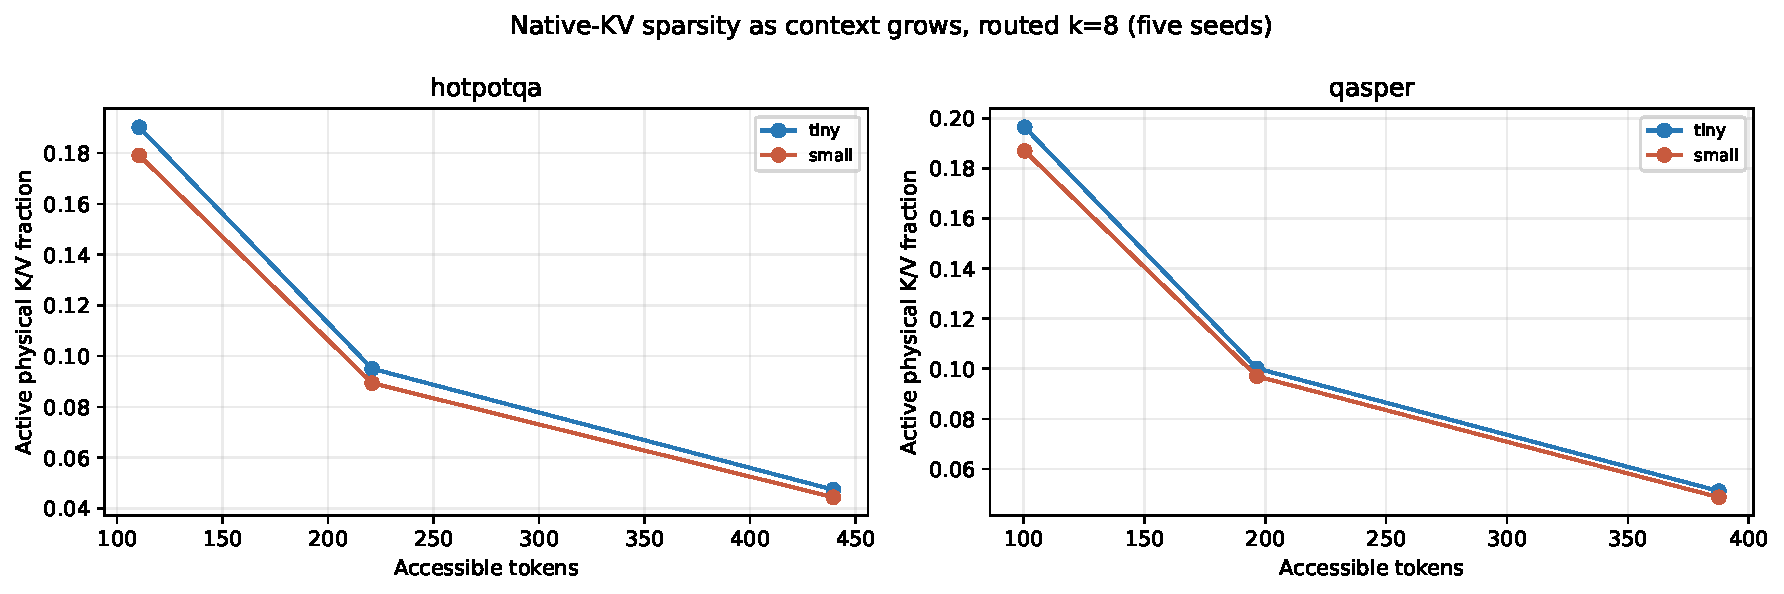
\includegraphics[width=.86\textwidth]{../shared/figures/pra_scale_sparsity.pdf}
\caption{\textbf{Fixed $k=8$ keeps physical selected K/V nearly flat as candidate memory
grows.} The resulting active fraction falls to 4.4--4.9\% at split 256 (255 source
units).}
\label{fig:scale-sparsity}
\end{figure}

\subsection{Fixed fraction: routing quality under equal sparsity pressure}

Fixed $k$ becomes progressively harsher: the selected candidate fraction changes from
12.7\% at split 64 to 6.3\% at split 128 and 3.1\% at split 256.
Reading the complete ranking at the cutoff nearest 12.5\% removes that confound.
Coverage remains 0.756/0.772/0.762 for HotpotQA-derived text and 0.794/0.803/0.800 for
QASPER-derived text. Figure~\ref{fig:fixed-fraction} shows every measured point;
no values are interpolated.

\begin{figure}[H]
\centering
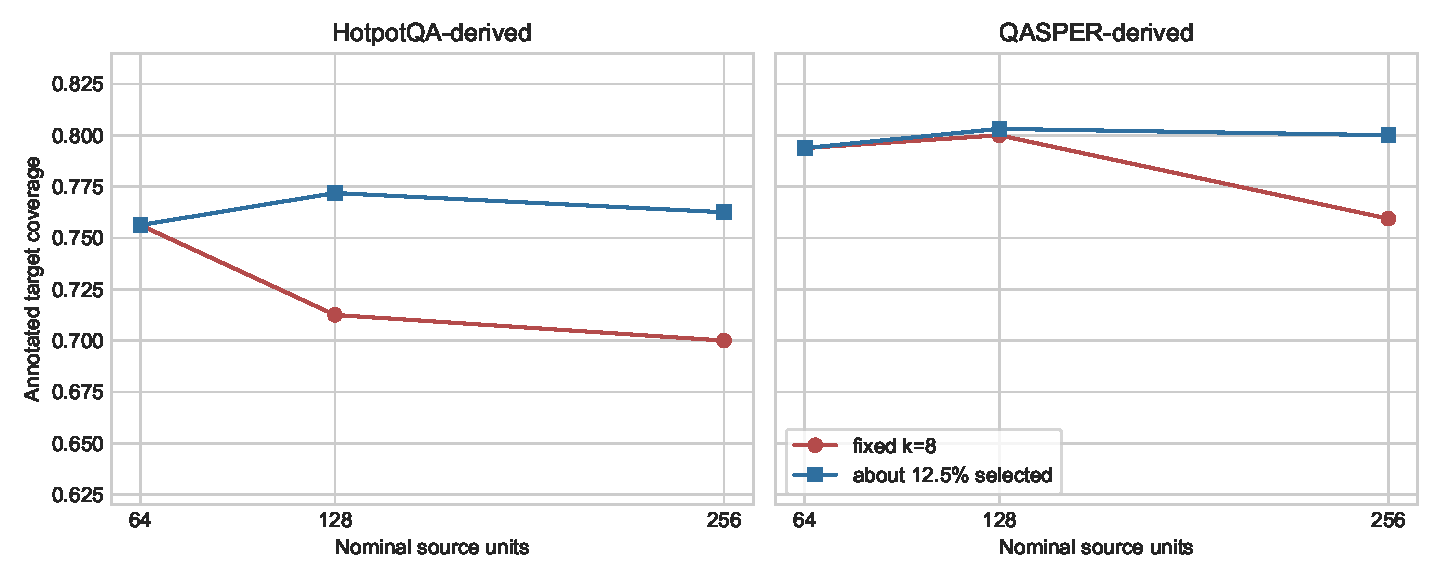
\includegraphics[width=.88\textwidth]{../shared/figures/pra_fixed_k_vs_fraction_scaling.pdf}
\caption{\textbf{Fixed-$k$ decline partly reflects increasing sparsity,
not intrinsic routing
collapse.} Holding selection near 12.5\% yields stable annotated target coverage through
the
measured split-256 scale.}
\label{fig:fixed-fraction}
\end{figure}

RCB and coverage answer different questions. RCB asks whether the selected K/V is
sufficient for this controlled prediction. Coverage asks whether the annotated source
was selected. A model can recover the answer when redundant or correlated evidence is
present even if the annotated URI is absent. Accordingly,
the perfect measured RCB at $k=8$ should not be read as perfect routing.

The retained scale artifact contains seed-level aggregates but not the per-question
target-hit/miss loss rows needed to identify why RCB remains near one when annotated
coverage is incomplete. Historical contextual slicing can propagate an answer-code
signal into later states whose URI is not the annotated target,
and correlated/redundant text is another possible route.
The current evidence does not distinguish these explanations.
We therefore limit the claim to loss recovery on this answer-coded probe;
it is not evidence of semantic retrieval at natural-QA difficulty.
A causal follow-up must export per-question traces and rebuild downstream state after
changing or removing the answer-bearing source.

\subsection{Measured model-capacity effect}

The same QASPER-derived $k=8$ run separates transport from tested model capacity.
Tiny-tier routed RCB declines from 1.000 at split 64 to 0.908 at split 256,
while the small tier remains 1.000. Its target coverage at split 256 is also 0.388
versus 0.759. Increased capacity materially improves this measured high-scale operating
point, but two small tiers do not support extrapolation to large models or prove that
capacity alone solves routing.

\section{Model-Bounded Logical Context}
\label{sec:bounded}

The scaling experiments above show sparse access,
but they do not by themselves prove that every underlying operation respects a model
limit. We therefore impose a hard $L_{\max}=32$ token limit on every source-encoding and
decode operation. The direct tail uses 8 tokens, the memory budget is 20,
and 4 tokens are reserved for accounting safety. The logical prompt contains 192 tokens,
of which 184 form an implicit addressable head. Encoding uses 16-token cores with up to
four tokens of left context. The frozen per-call trace reports a maximum source-encoding
input of 20 tokens, a direct input of 8, an actual retained-memory maximum of 20,
and therefore a combined attention K/V axis of 28.
The four-token reserve is unused capacity, not participating K/V.
Thus 20 is the largest source input, while 28 (87.5\% of the declared limit) is the
largest attention operation.

\begin{figure}[H]
\centering
\fbox{\begin{minipage}{0.90\textwidth}
\centering
\textbf{Logical request: 192 tokens}\\[3pt]
184-token displaced \texttt{\#\_\_head} $+$ 8-token direct tail\\[5pt]
$\downarrow$ head encoded in bounded blocks (largest source call: 20 tokens)\\[4pt]
$\downarrow$ compact routing selects full-detail K/V under a 20-token memory
budget\\[4pt]
$\downarrow$ native attention constraint:
$8\ \text{direct} + L_M\ \text{selected} + 4\ \text{reserve} \leq 32$
\end{minipage}}
\caption{\textbf{A 192-token logical request executes with source inputs no longer than
20
tokens and a combined attention K/V axis no longer than 28 under the configured 32-token
limit.} Logical history, displaced head, direct tail, retained memory, and combined K/V
length are distinct quantities; the four-token reserve is unused capacity.}
\label{fig:bounded-head-path}
\end{figure}

\begin{table}[H]
\centering
\small
\caption{\textbf{Routed PRA improves on truncation while all measured native calls
remain
bounded.} Five seeds cover 80 held-out cases. Dense full context is a diagnostic outside
the
imposed deployment limit and the model's shorter training distribution.}
\label{tab:bounded}
\begin{tabular}{lrrr}
\toprule
Condition & Loss & Accuracy & Target recall \\
\midrule
Dense full diagnostic & 1.7145 & 0.5125 & -- \\
Tail truncation       & 1.2287 & 0.6500 & -- \\
Independent blocks   & 1.7089 & 0.6375 & 0.2625 \\
Shuffled/wrong memory& 1.1205 & 0.6375 & -- \\
Routed PRA            & 1.0567 & 0.6875 & 0.525 \\
Approximate oracle    & 0.8738 & 0.7125 & 1.000 \\
\bottomrule
\end{tabular}
\end{table}

Routed PRA improves loss by 0.1720 and accuracy by 3.75 percentage points relative to
truncation, while all native calls remain within the 32-token limit.
The approximate oracle shows remaining headroom. However,
shuffled memory also improves loss over truncation,
so this experiment demonstrates useful sparse access and bounded execution,
not complete content-causal retrieval.

Increasing the memory budget from 4 to 20 tokens raises target recall from 0.325 to
0.525 and reduces loss from 1.2416 to 1.0567. Figure~\ref{fig:bounded-budget} makes the
tradeoff explicit: the available materialization budget controls how much selected
full-detail K/V can enter the bounded operation.

\begin{figure}[H]
\centering
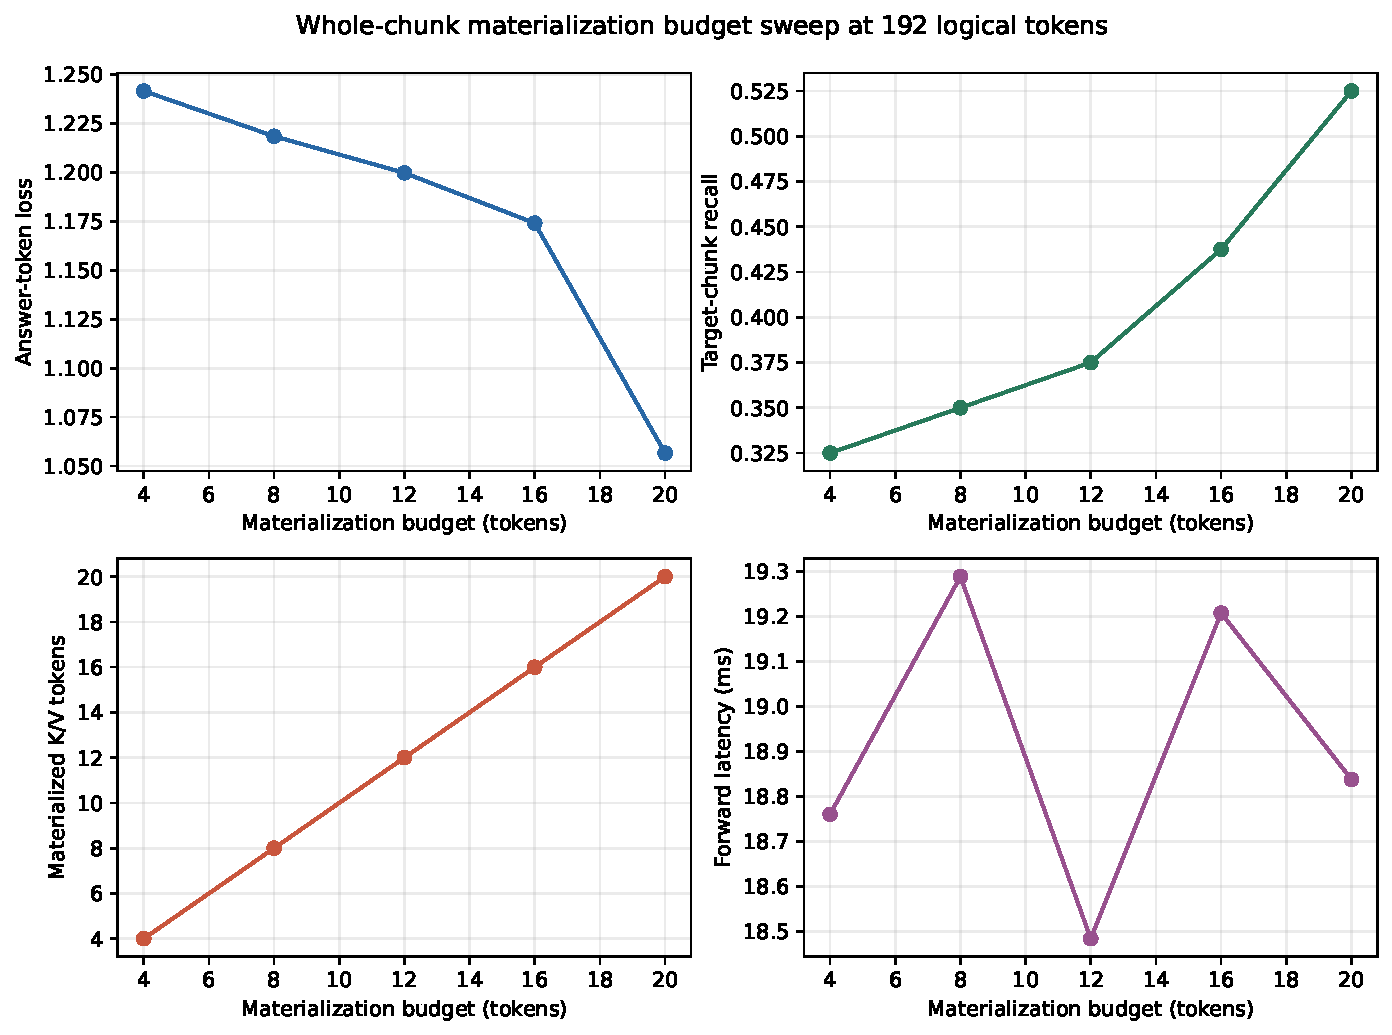
\includegraphics[width=.82\textwidth]{../shared/figures/pra_materialization_budget.pdf}
\caption{\textbf{The materialization budget exposes a quality--working-set frontier.}
Assigning
more of the 32-token operation budget to selected native K/V improves loss and target
recall.}
\label{fig:bounded-budget}
\end{figure}

The same mechanism supports rollover during generation.
In a 48-token generation smoke test, 11 rollovers migrate 44 historical tokens into
addressable memory while the largest source-encoding input remains 20 tokens and
combined attention remains at most 28. This verifies the state transition;
it is not a long-form generation quality result.

\section{Implementation and Systems Measurements}
\label{sec:systems}

The initial exact router repeatedly rebuilt Python objects and scored candidates in
loops. The packed implementation normalizes candidate gists once,
records offsets and ownership in tensors, and applies batched matrix products plus
\texttt{torch.topk}. At 256 candidates, warm exact search takes 5.49--6.28 ms in the
tiny tier and 11.46--11.56 ms in the small tier,
compared with 563--1183\,ms for the scalar path. The selected chunks are identical.
This 94--103$\times$ microbenchmark improvement demonstrates that exact routing need not
be Python-loop bound; it is not an end-to-end latency claim.

Persistent source K/V may also reside on CPU and move to the accelerator only after
selection. At split 256 (255 source units), this removes 0.734--3.420 MiB of measured
source K/V from GPU residency and transfers only 24.6--87.9 KiB per example.
The selected identities, materialized tokens, and loss match GPU-resident execution
exactly. Selective transfer itself takes 4.0--8.9 ms;
the complete warm-request path is 4.0--13.5 ms slower.
Index memory remains on GPU at 260 KiB in the tiny tier and 1.03 MiB in the small tier.
Figure~\ref{fig:kv-residency} also shows why source-K/V savings should not be confused
with whole-model peak allocation.

\begin{figure}[H]
\centering
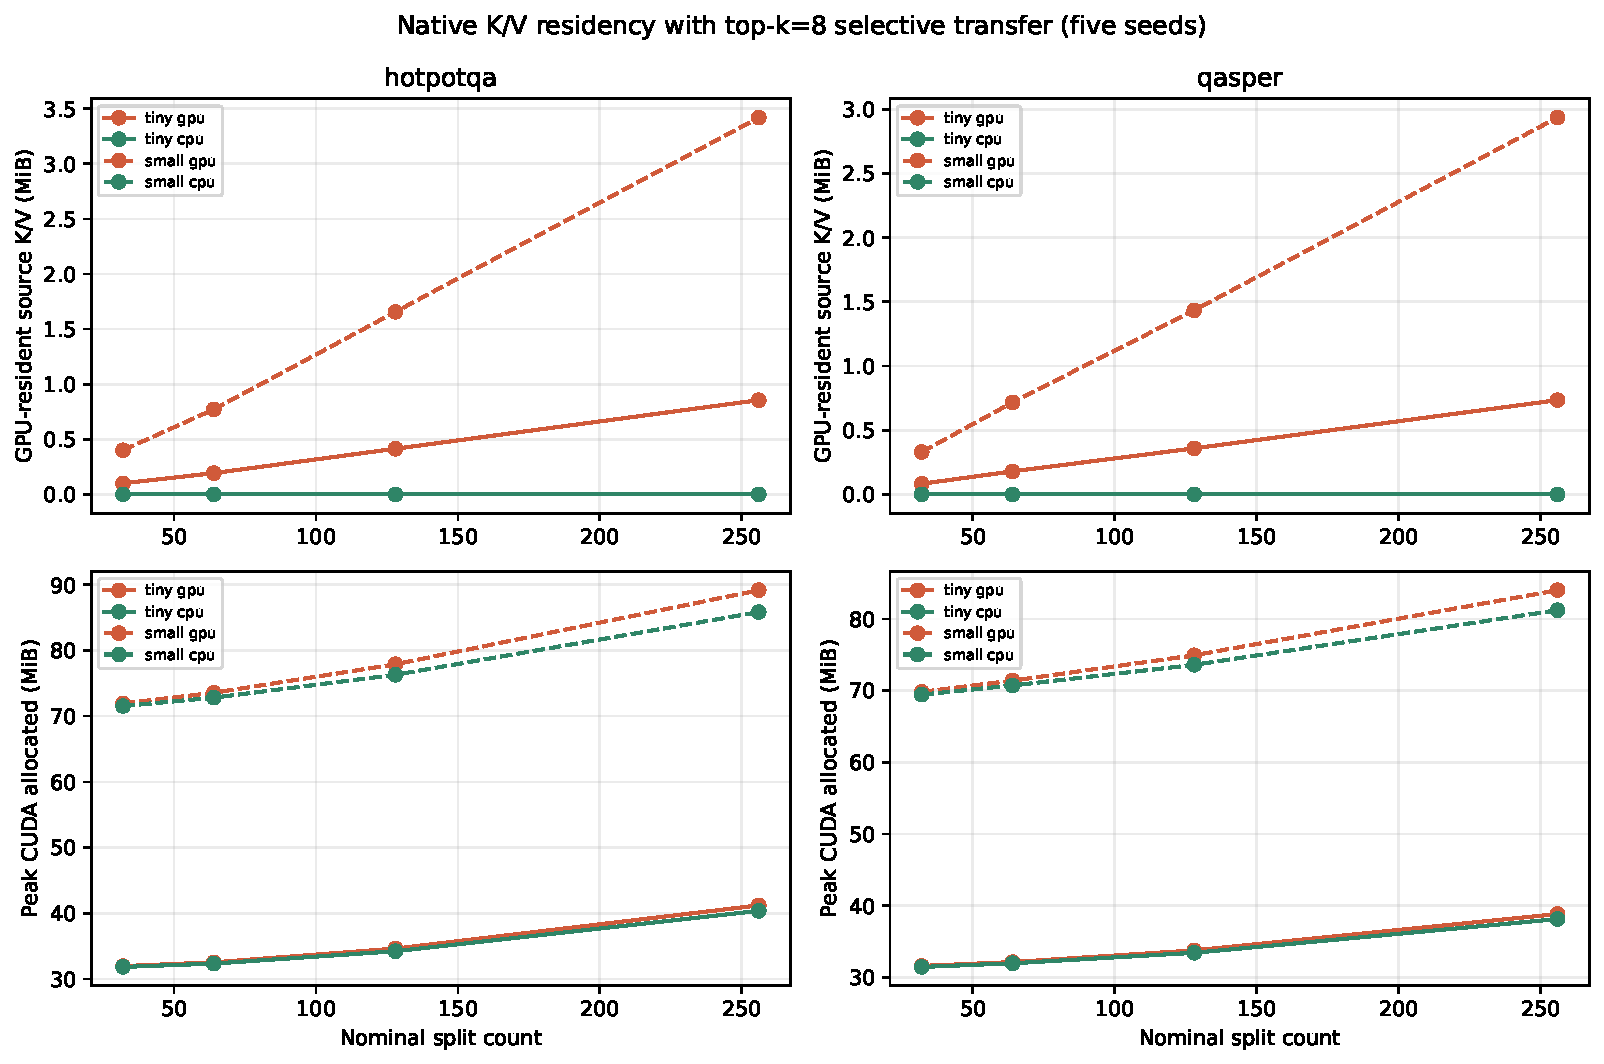
\includegraphics[width=.94\textwidth]{../shared/figures/pra_kv_residency.pdf}
\caption{\textbf{CPU residency removes the full inactive source cache from GPU while
preserving
the sparse selected payload.} At split 256 the measured saving is .734--3.420 MiB;
total peak
CUDA allocation falls less because model parameters and other tensors remain resident.}
\label{fig:kv-residency}
\end{figure}

\begin{table}[H]
\centering
\small
\caption{Systems measurements distinguish sparse-compute mechanics from unmeasured
production
serving claims.}
\label{tab:systems}
\begin{tabularx}{\textwidth}{l>{\raggedright\arraybackslash}X>{\raggedright\arraybackslash}X}
\toprule
Measurement & Established & Not established \\
\midrule
Exact packed routing &
  Split-256 (255-candidate) warm selection in 5.5--11.6 ms with scalar parity &
Production decode latency or approximate-index scaling \\
CPU-resident K/V & Lower GPU residency with identical selected state and loss &
Free storage or transfer-free attention \\
Bounded rollover & Continued generation without exceeding the declared operation limit &
Long-form generation quality \\
\bottomrule
\end{tabularx}
\end{table}

\section{Pretrained Scale and Context Dilution}
\label{sec:pretrained-dilution}

\paragraph{Pretrained calibration boundary.}
\textbf{This experiment tests transport compatibility and payload accounting in
pretrained
models; it does not evaluate PRA routing on these models.} The controlled experiments
above isolate mechanism, but they cannot answer whether a larger pretrained decoder
simply becomes insensitive to irrelevant context.
A separate MLX calibration therefore uses pinned 4-bit Qwen3-8B, 14B,
and 32B checkpoints on a 48~GiB M4 Pro. Five unique examples from each of QASPER,
HotpotQA, and 2Wiki provide frozen annotated evidence.
The same selection is rendered as at most 384 visible tokens for E0 and as native K/V
for E2, while deterministic same-dataset distractors extend the dense condition to 8K
source tokens. An 8B boundary sample extends three examples to 32K.
The requested 64K condition is recorded as
\texttt{NOT\_RUN\_MODEL\_CONTEXT\_LIMIT},
because the pinned checkpoints advertise 40,960
positions; no row is silently truncated.

\begin{table}[H]
\centering
\scriptsize
\caption{\textbf{Larger pretrained models do not make context dilution monotonic.}
$\Delta$ is full minus selected, so positive log-probability favors the full prompt. E2
agreement compares frozen selected native K/V with selected text.
Full MiB is the all-layer
native-K/V representation of the dense source, included to expose physical scaling
rather
than as a deployment recommendation.}
\resizebox{\linewidth}{!}{\begin{tabular}{llrrrrrr}
\toprule
Model & Context & $n$ & $\Delta$LP & $\Delta$F1 & E2 agr. & selected MiB & full MiB \\
\midrule
Qwen3-8B & 8K & 15 & +1.192 & +0.021 & 1.000 & 39.6 & 1152.0 \\
Qwen3-8B & 32K & 3 & -0.603 & +0.202 & 1.000 & 39.6 & 4608.0 \\
Qwen3-14B & 8K & 15 & -1.485 & -0.137 & 1.000 & 43.9 & 1280.0 \\
Qwen3-32B & 8K & 15 & -0.999 & -0.074 & 0.867 & 70.3 & 2048.0 \\
\bottomrule
\end{tabular}
}
\label{tab:pretrained-dilution}
\end{table}

\begin{figure}[H]
\centering
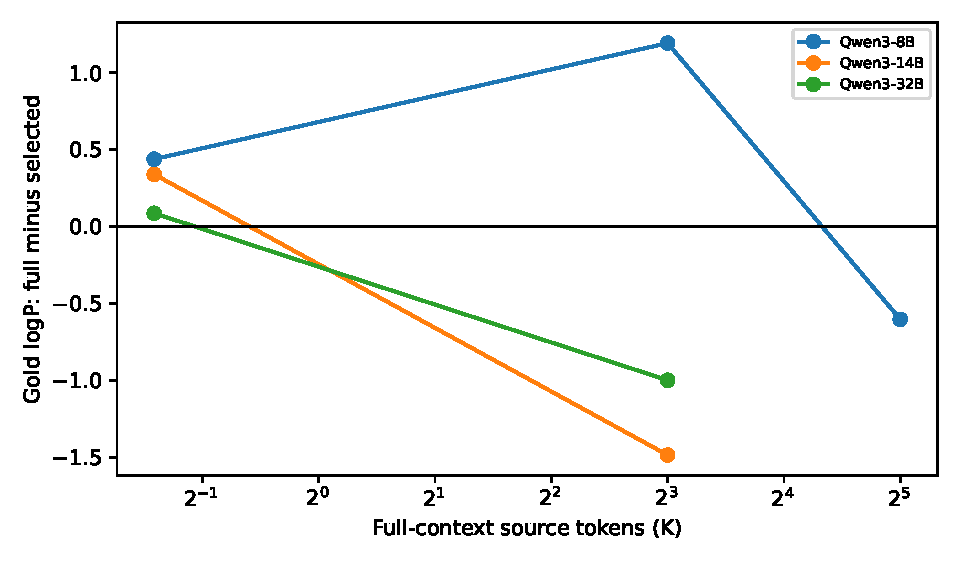
\includegraphics[width=.72\linewidth]{../shared/results/paper1_standalone_pra/mac_context_dilution/mlx_context_dilution.pdf}
\caption{Full-minus-selected answer log-probability changes sign across model size and
context. Selection bounds active evidence; it does not guarantee a quality advantage on
every question.}
\label{fig:pretrained-dilution}
\end{figure}

At 8K, full context improves mean gold-answer log probability by 1.192 nats at 8B but
lowers it by 1.485 nats at 14B and 0.999 nats at 32B.
F1 moves in the same direction for all three 8K cohorts, including 8B;
only the three-example 8B 32K boundary has likelihood and F1 moving in opposite
directions. The defensible result is therefore non-monotonicity,
not a universal selected-context quality gain. Larger models still require an explicit
dilution measurement.

The physical result is clearer. At 8B, selected all-layer native K/V remains about 39.6
MiB while full native K/V grows from 1,152 MiB at 8K to 4,608 MiB at 32K.
At 14B the corresponding 8K values are 43.9 and 1,280 MiB;
at 32B they are 70.3 and 2,048 MiB. Selected E2 preserves all sequences at 8B/14B and
13/15 at 32B, where its mean likelihood shift is only $+0.030$ nats.
Thus the bounded-working-set claim survives pretrained scale in this calibration even
though the quality sign depends on model and example.
It does not establish benchmark QA accuracy or a learned router at 8B--32B.

This is a shared MLX campaign with the companion positional study,
not an independent replication. Here it supports context-dilution and all-layer payload
accounting; coordinate and position-reset interventions are analyzed there.
E0 re-renders the frozen annotated selection as visible text,
whereas E2 injects native K/V sliced from the encoded selected layout.
Output-sequence agreement tests the consumer behavior of those two paths but does not
prove equality of every internal tensor. The MiB figures are serialized all-layer K/V
payload sizes, not measured peak unified-memory allocation or whole-process savings.

\section{Related Work by Changed Resource}

The useful comparison is not whether a method ``uses memory,'' but which resource it
changes: the external representation, attention graph, retained state,
recurrent summary, cache reuse, or active materialization.
Table~\ref{tab:related-resource-taxonomy} states these boundaries in one place.
The broader literature map appears in the companion survey;
this section makes the mechanical claim of Paper~1 independently readable.

\subsection{Retrieved text and neighbors}

RAG and REALM retrieve external text that is encoded for a reader or generator;
RETRO retrieves neighbor chunks and consumes them through chunked cross-attention
\cite{lewis2020rag,guu2020realm,borgeaud2022retro}.
Their shared strength is an updateable,
inspectable external corpus. PRA can compose with the same discovery layer,
but its immediate payload is different: selected information has already become
layer-native K/V and is restored inside native attention rather than reserialized as
prompt text. Consequently, RAG spends prompt or reader computation on selected text,
whereas Paper~1 budgets selected K/V tokens in a model operation.
Neither interface dominates the other; they move the external-to-active boundary at
different representations.

Text chunking also does not resolve PRA's fragmentation problem.
Retrieved passages are commonly encoded after selection and can interact in the reader.
PRA caches the contextual state for later activation,
so independently encoding each tiny routing unit irreversibly removes its preceding
context. This is why Section~\ref{sec:fragmentation} separates contextual encoding
blocks from fine routing views.

\subsection{Sparse, local, and block attention}

Longformer and BigBird prescribe sparse connectivity over an admitted sequence.
Reformer and Routing Transformer reduce attention cost through locality-sensitive
hashing or content-based clusters
\cite{beltagy2020longformer,zaheer2020bigbird,kitaev2020reformer,roy2021routing}.
These systems principally change which represented tokens interact.
Paper~1 instead separates the larger set of logically addressable objects from the
smaller set materialized for one operation. A sparse kernel could still execute the
admitted direct-plus-memory K/V, so graph sparsity and logical-memory sparsity are
complementary axes.

\subsection{KV retention, compression, and eviction}

H$_2$O, SnapKV, StreamingLLM, and ClusterKV retain selected positions from a stream
according to importance, an observation window, attention sinks, or clustered selection
\cite{zhang2023h2o,li2024snapkv,xiao2023streamingllm,liu2024clusterkv}.
KIVI instead reduces
bytes per retained K/V element through quantization~\cite{liu2024kivi}.
These methods change, drop, or more compactly represent the payload that remains
available. Paper~1 takes a conservative fidelity point:
its search metadata is compressed, but every selected payload is the stored full-detail
native K/V slice. Eviction and quantization can be layered underneath PRA,
but then their fidelity tradeoff must be reported separately from routing misses.

\subsection{External and latent memory}

Memorizing Transformer retrieves approximate-nearest-neighbor K/V from earlier examples,
while Landmark Attention trains landmark tokens to select blocks of an ingested context
\cite{wu2022memorizing,mohtashami2023landmark}. These are close architectural neighbors
because
they also narrow a large latent store before attention.
Paper~1 emphasizes a different access contract: application-addressable source identity,
compact per-chunk routing metadata, exact materialization of selected stored slices,
recorded source coordinates, and an explicit native-token budget.
Landmark blocks remain positions in one ingested context,
while approximate K/V neighbors need not preserve a named source coordinate.
PRA's stored coordinates are part of the payload contract,
although position transformation and extrapolation are deliberately left to Paper~1.5.
The distinction is therefore a combination of state type, addressing,
positional assumptions, lifecycle, and accounting,
not a claim that latent retrieval or block selection first appears here.

\subsection{Recurrent and summarized state}

Transformer-XL carries a bounded chronological activation memory across segments,
and Compressive Transformer compacts older activations into a coarser store
\cite{dai2019transformerxl,rae2020compressive}. Infini-attention and Feedback Attention
Memory
likewise maintain bounded recurrent or associative state
\cite{munkhdalai2024infini,hwang2024fam}. These approaches make long history usable by
carrying
or summarizing state as the sequence advances. PRA instead keeps separately addressable
regions and restores selected token detail. It pays external storage and routing cost to
avoid forcing all history through one recurrent summary;
recurrent methods avoid that object lifecycle but may superpose or compress old detail.

\subsection{Prompt and context caching}

PagedAttention manages physical KV blocks for serving.
Prompt Cache reuses schema-defined prompt modules,
while CacheBlend selectively recomputes reused chunk state to repair composition
\cite{kwon2023vllm,gim2023promptcache,yao2024cacheblend}. These systems primarily change
allocation or repeated-prefill cost. Paper~1 changes semantic addressability and bounded
activation: a cache hit alone does not determine whether an object should enter the
current attention operation. The mechanisms can compose,
with a serving cache storing PRA objects and a PRA router determining which cached
objects become active.

RetrievalAttention is the closest stored-K/V comparison:
it builds an attention-aware vector index over CPU-resident K/V and retrieves a small
token subset during decoding
\cite{liu2024retrievalattention}. PRA does not claim precedence for K/V retrieval.
Its narrower
addition in this study is a named-source lifecycle with contextual-block encoding,
independently addressable routing views, whole-unit admission,
and explicit accounting of source inputs versus the final direct-plus-memory attention
axis. Conversely, this prototype does not match RetrievalAttention's optimized
approximate index or serving evidence. CacheBlend addresses the complementary failure
caused by independently constructed prefix caches by selectively recomputing state;
PRA's fragmentation repair instead encodes contiguous context before exposing smaller
read-only views.

\begin{table}[H]
\centering
\scriptsize
\setlength{\tabcolsep}{3pt}
\renewcommand{\arraystretch}{1.03}
\caption{Memory families by the resource they change.
Entries describe canonical mechanisms;
individual systems may combine several rows. ``Bound'' means an explicit bound on K/V or
state
active in one model operation, not merely a finite implementation limit.}
\label{tab:related-resource-taxonomy}
\begin{tabularx}{\textwidth}{P{0.14\textwidth}P{0.14\textwidth}P{0.14\textwidth}P{0.16\textwidth}P{0.11\textwidth}Y}
\toprule
Family &
  External scope &
  Search/index &
  Active payload &
  Active bound &
  Payload fidelity \\
\midrule
RAG / retrieved text &
  corpus text &
  passage or neighbor index &
  re-encoded text or encoder state &
  top-$k$ retrieval, reader dependent &
  source text preserved; latent state recomputed \\
Sparse/block attention &
  admitted sequence &
  fixed, hashed, or learned edges &
  native states on allowed edges &
  pattern dependent &
  token state retained; interactions omitted \\
KV retention/compression &
  stream cache &
  token/page importance or quantizer &
  retained or quantized K/V &
  cache/byte budget &
  omitted or quantized detail \\
Recurrent or summary memory &
  chronological history &
  temporal update or learned read &
  compressed latent state &
  fixed recurrent state &
  history summarized or superposed \\
Latent/block retrieval &
  ingested or historical latent store &
  landmark, gist, or K/V index &
  selected hidden/native state &
  selected-block budget varies &
  method dependent \\
Prompt/context cache &
  reusable prompt modules &
  identity/schema lookup &
  cached attention state &
  serving policy dependent &
  exact reuse or selective repair \\
Paper~1 PRA &
  named logical sources &
  compact chunk gists &
  selected full-detail native K/V &
  hard native-token budget &
  selected payload unchanged \\
\bottomrule
\end{tabularx}
\end{table}

\subsection{Novelty boundary and companion scope}

Paper~1 contributes the combination visible in the last row: addressable logical memory,
compact routing metadata, selected full-detail layer-native K/V,
a hard native-operation bound, and separate encoding and routing granularity.
It does not claim precedence for each component in isolation,
nor does it establish production superiority over the neighboring families.

Position assignment, RoPE rebinding, and the difference between attention and semantic
routing geometry belong to companion Paper~1.5~\cite{simao2026position}.
Exact retrofit into pretrained Hugging Face model families and its adaptation/behavioral
evaluation belong to companion Paper~2~\cite{simao2026hf}.
This paper owns the narrower standalone mechanism:
logical memory can exceed active native K/V under a hard model-operation bound while
selected payload remains full-detail native state.

\section{Limitations, Safety, and Scope}
\label{sec:limitations}

The evidence is controlled. Models are small, targets are synthetic or answer-coded,
and the natural-text probes are not unrestricted HotpotQA or QASPER evaluation.
Five paired seeds establish directional consistency but offer limited statistical
resolution. At five pairs, the smallest attainable exact two-sided sign-flip result is
$p=0.0625$.

The pretrained dilution calibration narrows one scale limitation but does not remove it.
It has 15 independent examples per 8K model point, only three at 32K, one Qwen family,
one quantization, and no 64K execution. Repeated generation is not counted as additional
quality evidence, and its annotated selector does not validate learned large-model
routing.

Routing quality remains the main unresolved issue.
Stable fixed-fraction target coverage through split 256 (255 source units) is
encouraging, but coverage near 0.76--0.80 leaves substantial room for better selectors.
The bounded-context router reaches only 0.525 recall,
and the shuffled control shows that some gain is not source-specific.
PRA makes sparse access possible; it does not make relevance estimation automatic.

Sparse selection alone reduces active attention, not necessarily GPU residency.
If every inactive detail tensor remains on the accelerator,
the external cache still grows with logical memory.
The CPU-residency experiment measures one offload tradeoff,
but it does not establish production transfer efficiency, asynchronous overlap,
or arbitrary memory scale. Logical-memory support is likewise not dense full-context
equivalence: unselected K/V is absent from the operation.

Position semantics are another independent constraint.
Preserving source coordinates is necessary for the standalone absolute-position
experiments, but this paper does not claim that a pretrained positional geometry
extrapolates to arbitrary logical offsets. The companion position paper studies
RoPE-aware integration. Pretrained Hugging Face adapters, iterative multi-hop retrieval,
multiple gists per chunk, and production serving are outside this paper's evidence.

External K/V is sensitive derived state. Implementations must bind cache entries to
request and authorization scope, prevent URI collisions across batch rows,
define invalidation and retention, and avoid exposing routing traces across tenants.
Implicit prompt-head memory is request-local even when every request uses the same
internal name.

\section{Conclusion}

PRA separates addressable logical memory from the native K/V active in one transformer
operation. Contextual encoding can remain coarse enough to preserve historical state
while routing views remain fine enough for sparse selection.
The gist is routing metadata; the selected full-detail K/V is the attention payload.

The controlled evidence establishes two observed fixed-budget trends through split 256
(255 addressable source units). At fixed $k$, physical selected K/V remains nearly flat
and the active fraction falls to 4.4--4.9\%. At a fixed selection fraction,
target coverage remains stable near 0.76--0.80. A 192-token logical prompt also executes
under a hard 32-token native limit, and CPU residency converts sparse selection into
measured GPU-cache savings without changing loss or selected state.

This controlled scope leaves routing, pretrained positional integration,
and optimized serving to future work. PRA nevertheless separates growing logical memory
from per-operation active K/V.

\appendix

\section{Secondary Ablations}
\label{app:ablations}

\paragraph{Selection breadth.}
Increasing $k$ improves coverage and raises active K/V.
The correct operating point is therefore a frontier, not a universal constant.
Fixed-$k$ comparisons should always report the realized fraction,
and fixed-fraction comparisons should disclose the measured $k$ chosen at each candidate
count.

\paragraph{Chunk overlap.}
Overlap can protect facts that cross routing boundaries,
but it duplicates physical K/V and makes selected-token accounting differ from
unique-token accounting. The main scaling tables report physical active tokens because
those are materialized by the prototype.

\paragraph{Wrong-memory controls.}
Disabled, shuffled, irrelevant, and oracle conditions serve different purposes.
Disabled memory measures the direct baseline; shuffled memory tests identity dependence
while preserving payload volume; irrelevant memory tests distractor sensitivity;
and oracle selection tests transport independently of routing. None alone is sufficient.

\section{Historical Cross-Attention Adaptation}
\label{app:adaptation}

An earlier V1 branch used a separately projected cross-attention-capable memory path.
It is retained here for provenance, not as the architecture evaluated in the main paper.
Across five paired seeds, freezing the pretrained backbone and adapting only that memory
path reduced reference-conditioned loss from 6.3557 to 4.6720 in the full-PRA variant
and from 6.3642 to 4.7296 in the hybrid variant.
It preserved plain-language losses exactly at 4.5034 and 4.5500;
direct joint tuning instead increased them by 0.1775 and 0.1562.

The result supports staged adaptation within that historical branch,
but it does not establish a general pretrained-model result.
Reference selection remained near chance (MRR 0.4202),
and shuffled/oracle deltas were very small. The native-KV experiments in
Sections~\ref{sec:transport}--\ref{sec:bounded} are the evidence for the present
mechanism.

\section{Minimal Reimplementation Guide}
\label{app:implementation}

The following pseudocode captures the default single-gist,
native-KV path evaluated in this paper. The source map refers to repository commit
\texttt{5b71e2e}; line numbers are pinned to that snapshot so later edits do not
silently move the referenced implementation.

\begin{verbatim}
encode_source(source, max_native_length):
    for contextual_block in bounded_contiguous_blocks(source):
        hidden = transformer(contextual_block)
        for layer in pra_layers:
            K, V = layer.project_kv(hidden[layer])
            commit_only_nonoverlapping_core(K, V, source_positions)
    for routing_chunk in views_over_committed_kv():
        gist = normalized_mean(routing_chunk.keys)
        index.add(gist, kv_offsets, owner)

attend(query, direct_kv, memory_budget):
    scores = packed_normalized_gists @ normalize(query)
    ranked = exact_topk(scores)
    selected = admit_whole_chunks(ranked, memory_budget)
    memory_kv = gather_original_native_kv(selected)
    assert len(direct_kv) + len(memory_kv) + reserve <= native_limit
    return attention(query, concat(memory_kv, direct_kv))
\end{verbatim}

\begin{table}[H]
\centering
\small
\caption{Code map for an independent implementation. Line ranges refer to commit
\texttt{5b71e2e}.}
\label{tab:code-map}
\begin{tabularx}{\textwidth}{l l X}
\toprule
Concern & Source lines & Role \\
\midrule
Native K/V projection & \texttt{attention.py:89--130} & Reuse a layer's existing key and
value projections without a separate memory projection. \\
Budget and materialization &
  \texttt{attention.py:155--329} &
  Admit whole selected chunks,
gather their token K/V, and account for overlap and timing. \\
Direct + memory attention & \texttt{attention.py:331--430} & Concatenate selected memory
with direct K/V under one score normalization and output projection. \\
Packed exact index & \texttt{memory.py:457--639} & Normalize and pack gists, preserve
ownership and offsets, and score candidates tensorially. \\
Selection semantics &
  \texttt{memory.py:947--1188} &
  Apply breadth, hierarchy, and stable
ranking rules and serialize traces. \\
Bounded source encoding &
  \texttt{model.py:430--630} &
  Encode contiguous blocks with left
context and commit only each block's core state. \\
Cache construction & \texttt{model.py:631--900} & Partition registered sources, generate
gists, and associate routing views with layer-native K/V. \\
Row-private batch cache & \texttt{memory.py:1217--1306} & Keep reference ownership and
implicit heads isolated between batch rows. \\
\bottomrule
\end{tabularx}
\end{table}

An implementation should pass four tests before quality evaluation:
memory-disabled PRA must match its SelfAttention source model;
native-all memory must match dense-context tail logits where the position regime is
valid; oracle selection must transport the target state;
and packed routing must return the same ordering as a scalar exhaustive implementation.
It should then report candidate count, realized selection fraction,
physical and unique K/V tokens, target coverage, operation length,
index-build and warm search time, transfer bytes, and row ownership.

{\small
\bibliographystyle{plain}
\bibliography{../shared/references}
}

\end{document}
